% Of course, if you prefer, you can just start with
%   \chapter{My First Chapter Name}
% and start typing away.
\chapter{The Many Flavors of the Periodicity Transform}
Since Sethares, the PT has been developed in multiple directions. This chapter concerns itself with the examining and presenting existing versions and their potential applicability to audio analysis and synthesis.

\section{Nonorthogonal Periodic Decomposition}
    Sethares and Staley:

    A sequence of real numbers $x(k)$ is called $p$-periodic if there is an integer $p$ with $x(k+p) = x(k)$ for all integers $k$. In practice, we will consider signals of finite length $N$, which are always periodic with period $P_N$. Smaller periodicities are found by projecting $x_N$ onto the subspaces $P_p$ for $p < N$. When $x_N$ is “close to” a periodic subspace $P_p$ then there is a $p$-periodic element $x_p$ that is contained within $x_N$. The fundamental formula for projection is:
    \begin{equation} \label{eq:proj}
      \alpha_s = \frac{1}{\lfloor N/p \rfloor} \sum_{n=0}^{\lfloor N/p \rfloor -1} x_{N_i} (s + np)
    \end{equation}
    where $N_i = p \lfloor N/p \rfloor$ to deal with partial sequences.\footnote{This is slightly modified in this paper, described in Section \ref{wholeperiods}.} Most notably, this transform works only with \emph{integer} periods.

    % \begin{equation}
    %   \delta_p^s(j) =
    %   \left\{ \begin{array}{l}
    %   1, \text{ if }(j-s)\text{ mod }{p=0} \\
    %   0, \text{ otherwise.}
    %    \end{array} \right.
    % \end{equation}
    % where $s$ is the “time shift” so that $s = [0,1,2,...,p-1]$

    \subsection{An Example}
    This process is most easily understood in the context of a short example. Let $x = \{ ... , 2, -1.1, -1.1, 2,$
    $-1.2, -1.2, 2, -1.1, -1.1, 2, -1.2, -1.1, 2, -1.1,...\}$ where $N = 14$. The signal is plotted in Figure \ref{fig:firstSig_proj} in blue. Let $p = 3$ which means $s = \{0,1,2\}$. For $s=0$:
    $$
    (s + np) = [1, 4, 7, 10, 13]
    $$
    $$
    x(s + np) = [2,2,2,2,2]
    $$
    Therefore:
    $$
    \alpha_0 = \frac{1}{\lfloor 14/3 \rfloor} \sum_{n=0}^{\lfloor 14/3 \rfloor -1} x(s + np) = 2
    $$
    Then replace all values at indicies $(s+np)$ with 2, giving $[2,2,2,2,2]$. Similarly, $\alpha_1 = [-1.14,-1.14,-1.14,-1.14, -1.14]$ and $\alpha_2 = [-1.125,-1.125,-1.125,-1.125]$. Interleaving the results, we find $x_3 = \{..., 2, -1.14, -1.125,...$
    $\}$. This projection is plotted over the original signal in the bottom of Fig.1.

    \begin{figure}[h]
      \centering
      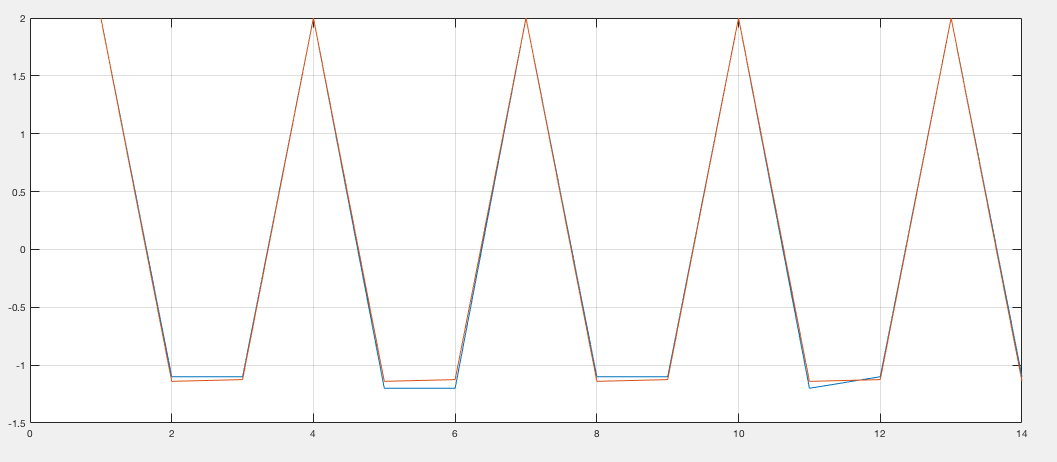
\includegraphics[width=1\textwidth]{chapters/01/figs/firstSig_proj.png}
      \caption[Sethares and Staley's periodicity transform overlayed.]
    {The periodicity transform of Sethares and Staley. \index{firstSig_proj}}
      \label{fig:firstSig_proj}
    \end{figure}

    More generally,
    \begin{equation} \label{eq:pixp}
      x_p = \pi(x, P_p) = \sum_{s=0}^{p-1} \alpha_s \delta_p^s
    \end{equation}

    where, $\pi(x, P_p)$ represents the projection of $x$ onto $P_p$, $\delta_p^s$ are the $p$-periodic basis elements of $P_p$, and $s$ is as defined above. (\ref{eq:pixp}) describes the method of projection used in this paper and the M-best $\gamma$ algorithm. Of note is the fact that these periodic basis vectors as acquired by (\ref{eq:pixp}) are \emph{not} orthogonal. Muresan and Parks in \cite{muresan2003orthogonal} presented a method of finding orthogonal periodic basis vectors but their method was not implemented for this paper (and may in fact be unncessary when resynthsizing audio).



\section{Orthogonal Periodic Decomposition}

Orthogonal decomposition of Muresan and Parks.

\section{Ramanujan Periodic Decomposition}

Vaidyanathan and Tenneti
